\documentclass[11pt]{article}

\usepackage[T1]{fontenc}
\usepackage[utf8]{inputenc}
\usepackage{lmodern}
\usepackage{microtype}
\usepackage{graphicx}
\usepackage{xcolor}
\usepackage{float}
\usepackage{booktabs}
\usepackage{longtable}
\usepackage{tabularx}
\usepackage{array}
\usepackage{enumitem}
\usepackage[margin=0.86in]{geometry}
\usepackage[hidelinks]{hyperref}

\definecolor{atlasink}{HTML}{071923}
\definecolor{atlascyan}{HTML}{168F9D}
\definecolor{atlasgold}{HTML}{C99A3D}
\definecolor{atlasseal}{HTML}{B84A3A}
\definecolor{atlasmuted}{HTML}{607779}

\hypersetup{
  pdftitle={From Neural Computation to Multimodal Remote Sensing Intelligence},
  pdfauthor={Licheng Jiao Research Atlas Project},
  pdfsubject={A systematic data-driven review of Licheng Jiao's research landscape, 1998--2026},
  pdfkeywords={Licheng Jiao, remote sensing, evolutionary optimization, computer vision, bibliometrics, systematic mapping}
}

% LaTeXML recognizes the alt key. This no-op definition keeps pdfLaTeX
% compilation portable while preserving explicit alternative descriptions.
\makeatletter
\define@key{Gin}{alt}{}
\makeatother

\setlist[itemize]{leftmargin=1.3em,itemsep=0.35em}
\setlist[enumerate]{leftmargin=1.5em,itemsep=0.45em}
\renewcommand{\arraystretch}{1.16}
\setlength{\emergencystretch}{2em}

\newcommand{\evidenceboundary}{%
  \begin{center}
  \fcolorbox{atlascyan}{white}{%
    \begin{minipage}{0.92\linewidth}
    \textbf{\textcolor{atlascyan}{Evidence boundary.}}
    The current public catalog does not contain source-verified abstracts or
    full text for the complete corpus. This review supports bibliometric and
    title-level systematic mapping; it does not infer experimental superiority,
    numerical performance, or technical novelty from titles alone.
    \end{minipage}}
  \end{center}
}

\newcommand{\figureqr}[2]{%
  \begin{flushright}
  \begin{minipage}{0.22\linewidth}
  \centering
  \includegraphics[width=0.68\linewidth,alt={QR code opening the full-resolution #1 figure.}]{qr/#2.png}\\[-0.2em]
  {\scriptsize\textcolor{atlasmuted}{Scan for full-resolution figure}}
  \end{minipage}
  \end{flushright}
}

\title{\textbf{From Neural Computation to Multimodal Remote Sensing Intelligence}\\[0.5em]
\large A Systematic, Data-Driven Review of Licheng Jiao's Research Landscape, 1998--2026}
\author{Licheng Jiao Research Atlas Project}
\date{Data snapshot: 28 July 2026}

\begin{document}

\maketitle

\begin{abstract}
This review maps the scholarly landscape associated with Licheng Jiao using
1,827 bibliographic records spanning 1998--2026. The corpus is anchored to the
DBLP author profile 40/3714 and DOI-linked public metadata. We introduce a
reproducible hierarchy of seven broad domains and 48 observed research tasks,
reconstruct four phases of research evolution, identify corpus-scoped first
appearances at selected journals and conferences, and analyze collaboration and
Crossref Cited-by evidence. The synthesis suggests a durable research logic
connecting structure-aware representation, adaptive search, intelligent
perception, and domain-grounded interpretation. Contemporary multimodal and
foundation-model work is therefore interpreted as a recombination of earlier
methodological commitments rather than an isolated turn. Evidence boundaries
remain explicit: this release is a bibliometric and title-level systematic
mapping, not a substitute for source-verified full-text review.
\end{abstract}

\section{Introduction}

Long research careers are difficult to summarize with a short list of
``representative papers.'' Such lists are readable, but they hide continuity,
collaboration, and the movement of methods across application domains. This
review instead treats the publication record as a longitudinal research system.
Its central question is how a program rooted in neural computation,
evolutionary search, and multiscale signal analysis expanded into visual
intelligence, remote-sensing interpretation, and contemporary multimodal
models.

The presentation adopts the useful discipline of modern systems surveys:
define the object and scope, disclose the corpus protocol, provide an overview
map before detailed taxonomy, reconnect categories through cross-cutting
synthesis, and close with testable open questions
\cite{li2026harness,ren2026selfimprovement}. The visual language is original
and generated from this corpus; the cited surveys serve as organizational
references, not sources for copied figures or claims about Licheng Jiao's work.

\subsection{Contributions}

This review makes four contributions.

\begin{enumerate}
\item \textbf{Reproducible corpus construction.} DBLP identity anchoring, DOI
linkage, public field allowlists, and versioned generation scripts make every
reported count inspectable.
\item \textbf{Hierarchical systematic mapping.} Seven broad domains and 48
observed tasks connect 1,827 records while keeping the title-level coding rules
visible.
\item \textbf{Longitudinal synthesis.} Four phases and selected first-venue
milestones show when methodological and institutional frontiers enter the
public corpus.
\item \textbf{Relational evidence.} Collaboration, venue, and Crossref citation
layers complement topic counts and establish questions for a later,
source-verified full-text review.
\end{enumerate}

\section{Corpus and Review Protocol}

\subsection{Identity anchor and unit of analysis}

The corpus uses the DBLP author profile \texttt{40/3714}
\cite{dblp-jiao} as its identity anchor. DOIs and DBLP keys support
record-level verification. The snapshot contains 1,827 records from 1998
through 2026, including 1,764 DOI-bearing entries. Counts refer to
bibliographic records rather than deduplicated intellectual works; conference,
preprint, and journal versions may therefore coexist.

\begin{table}[ht]
\centering
\caption{Corpus summary for the July 2026 snapshot.}
\label{tab:corpus}
\begin{tabular}{lr@{\hspace{2.8em}}lr}
\toprule
Measure & Value & Measure & Value \\
\midrule
Bibliographic records & 1,827 & Journal records & 1,369 \\
Conference records & 453 & Proceedings records & 5 \\
Records with a DOI & 1,764 & Observed year range & 1998--2026 \\
Distinct coauthors & 2,163 & Distinct venues & 260 \\
Broad domains & 7 & Observed fine tasks & 48 \\
\bottomrule
\end{tabular}
\end{table}

\subsection{Collection, inclusion, and exclusion}

Records are included when they are traceable to the selected DBLP profile.
Bibliographic fields are normalized into a strict public schema: stable ID,
title, authors, year, publication type, venue, pages or volume, DOI, DBLP key,
and public URLs. Local download state, credentials, machine paths, private
annotations, and raw working logs are excluded. This separation protects the
public website boundary and prevents operational metadata from being mistaken
for scholarly evidence.

\subsection{Hierarchical coding protocol}

Each title and venue string is processed by ordered, human-readable keyword
rules. The first level assigns one of seven broad domains: frontier models and
multimodality, remote-sensing interpretation, visual perception, evolutionary
optimization, neural and machine learning, signal and computational imaging,
or interdisciplinary methods and applications. The second level assigns a
more specific task, such as SAR interpretation, hyperspectral classification,
change detection, multiobjective optimization, neural architecture search,
segmentation, tracking, image restoration, or vision--language prompting.

This procedure favors auditability over opaque clustering. It is deterministic
and easy to challenge, but a single-label taxonomy necessarily compresses
hybrid work. Counts should therefore be read as navigational coordinates, not
as an official classification supplied by the researcher.

\subsection{Citation, collaboration, and first-venue measures}

Citation counts are retrieved by DOI from Crossref Cited-by
\cite{crossref-citedby}. Crossref counts depend on references deposited into
its network and may under-report the complete citation record. Coauthor counts
represent record-level co-occurrence after name normalization; they do not
measure contribution, seniority, or supervision.

Selected venue milestones are generated by exact or documented venue-family
matching. ``First'' means the earliest matching year in this DBLP-anchored
corpus. When multiple records share that first year, all are grouped rather
than assigned a false within-conference chronology.

\evidenceboundary

\section{A Unifying View of the Research Program}

The corpus supports a four-layer interpretation of the research program.
\emph{Structure-aware representation} describes repeated attention to
multiscale, sparse, spectral--spatial, geometric, and attentive
representations. \emph{Adaptive search and optimization} captures evolutionary,
multiobjective, transfer, and architecture-level search. \emph{Intelligent
perception} includes classification, detection, segmentation, tracking,
restoration, and matching. Finally, \emph{domain-grounded interpretation}
reflects sustained engagement with SAR, PolSAR, hyperspectral, aerial, and
satellite data.

\begin{figure}[H]
\centering
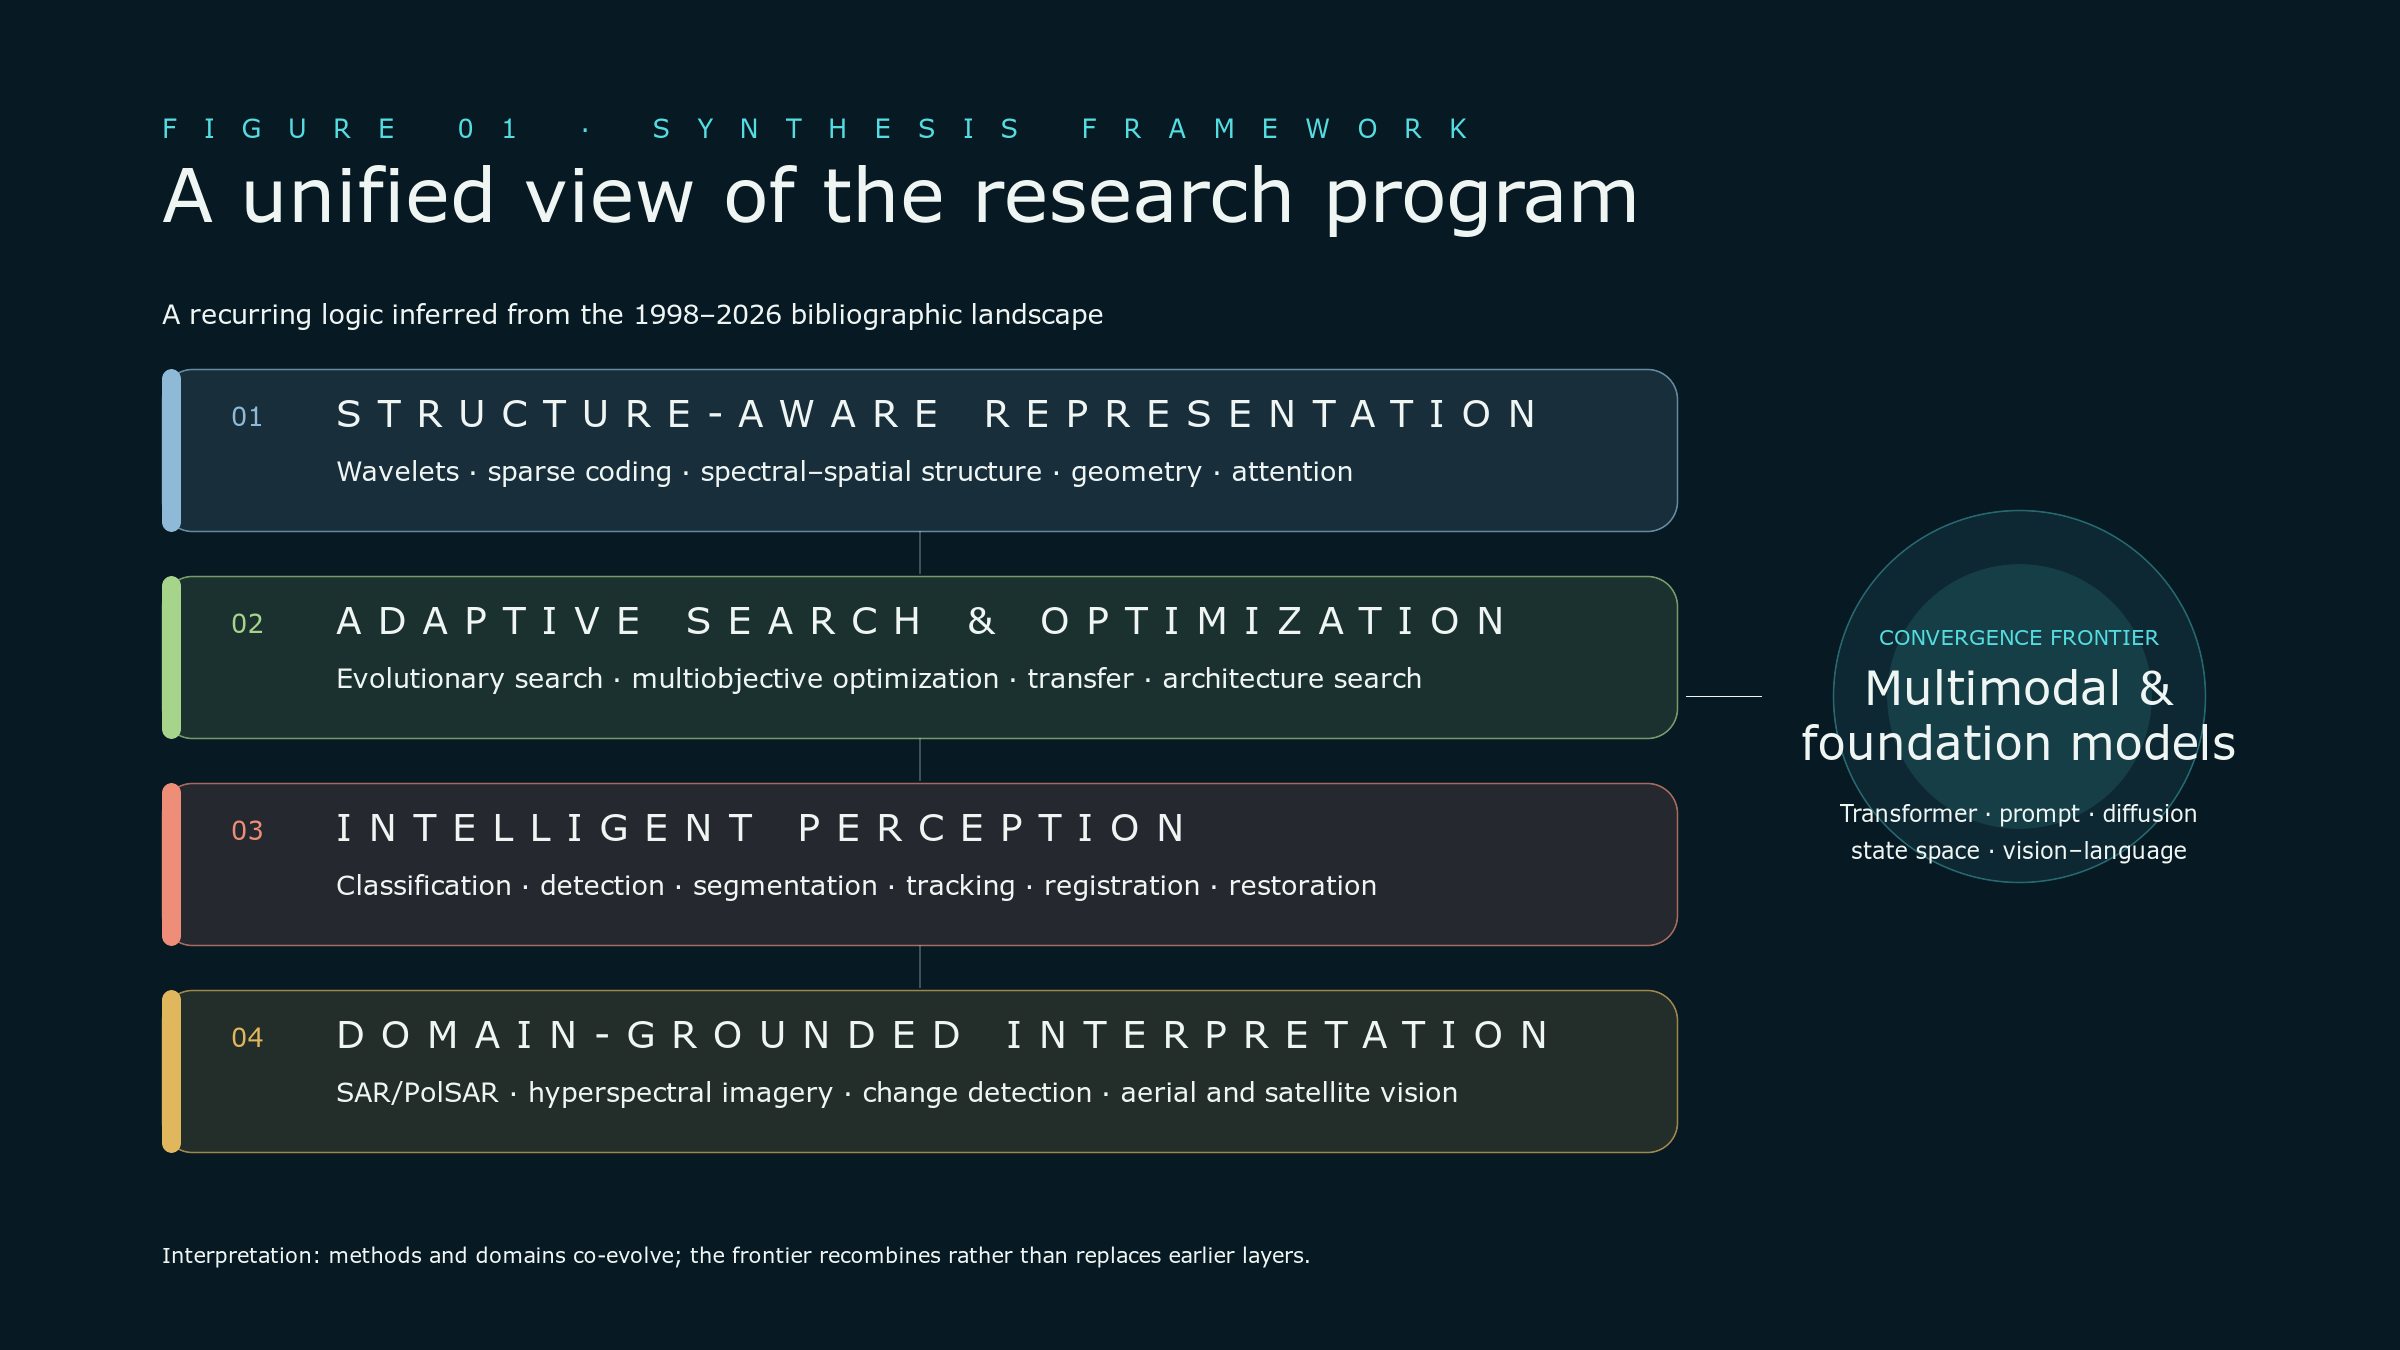
\includegraphics[width=\linewidth,alt={Four-layer framework connecting structure-aware representation, adaptive search and optimization, intelligent perception, and domain-grounded interpretation to a multimodal and foundation-model convergence frontier.}]{figures/research-program-framework.png}
\caption{Original synthesis framework for the research program. The diagram
summarizes recurring methodological relations inferred from the bibliographic
landscape; it is not an author-supplied taxonomy.}
\label{fig:framework}
\figureqr{research-program framework}{research-program-framework}
\end{figure}

These layers are not historical stages. They interact across time:
remote-sensing constraints motivate new representations; search procedures
choose features and architectures; perception tasks provide demanding
evaluation settings; and modern multimodal systems recombine all four. The
framework therefore interprets the contemporary frontier as convergence rather
than replacement.

\subsection{Structure-aware representation}

Early multiscale and wavelet work, sparse representations, spectral--spatial
modeling, geometric matching, attention, and recent state-space architectures
share a concern with how structure is represented. The techniques differ
substantially, but the bibliographic trajectory repeatedly returns to the
premise that signals and images should be modeled through meaningful
relations---across scale, spectrum, space, geometry, or time.

\subsection{Adaptive search and optimization}

Evolutionary computation is not confined to a historical period. It appears in
multiobjective search, feature and band selection, scheduling, clustering,
architecture search, and large-scale optimization. Highly cited examples such
as MOEA/D with adaptive weight adjustment \cite{qi2014moead}, Two\_Arch2
\cite{wang2015twoarch}, and decision-variable analysis for large-scale
optimization \cite{ma2016largevariables} illustrate the visibility of this
methodological axis.

\subsection{Intelligent perception and domain grounding}

Classification, detection, segmentation, tracking, matching, registration, and
restoration form the perception layer. Remote sensing supplies a sustained
domain context whose multiscale, multimodal, and physically grounded data
challenge generic vision assumptions. Change detection in SAR imagery
\cite{gong2016sarchange}, spectral--spatial hyperspectral modeling
\cite{zhu2021ressan}, and image registration \cite{ma2017registration} are
prominent examples in the citation landscape.

\section{Longitudinal Evolution and Venue Frontiers}

\subsection{Four phases}

The publication trajectory can be summarized in four phases.

\begin{description}[leftmargin=3.2cm,style=multiline]
\item[1998--2007: 179 records] Neural networks, evolutionary computation,
clustering, wavelets, and early pattern recognition establish a methodological
base.
\item[2008--2014: 293 records] Multiobjective optimization, sparse
representation, imaging, SAR, and remote-sensing classification become
increasingly connected.
\item[2015--2020: 530 records] Deep visual learning expands across
hyperspectral data, change detection, scene recognition, detection,
segmentation, and multimodal fusion.
\item[2021--2026: 825 records] Transformers, prompts, vision--language
interaction, diffusion, Mamba, state-space models, and foundation-model
adaptation recombine earlier themes.
\end{description}

\begin{figure}[H]
\centering
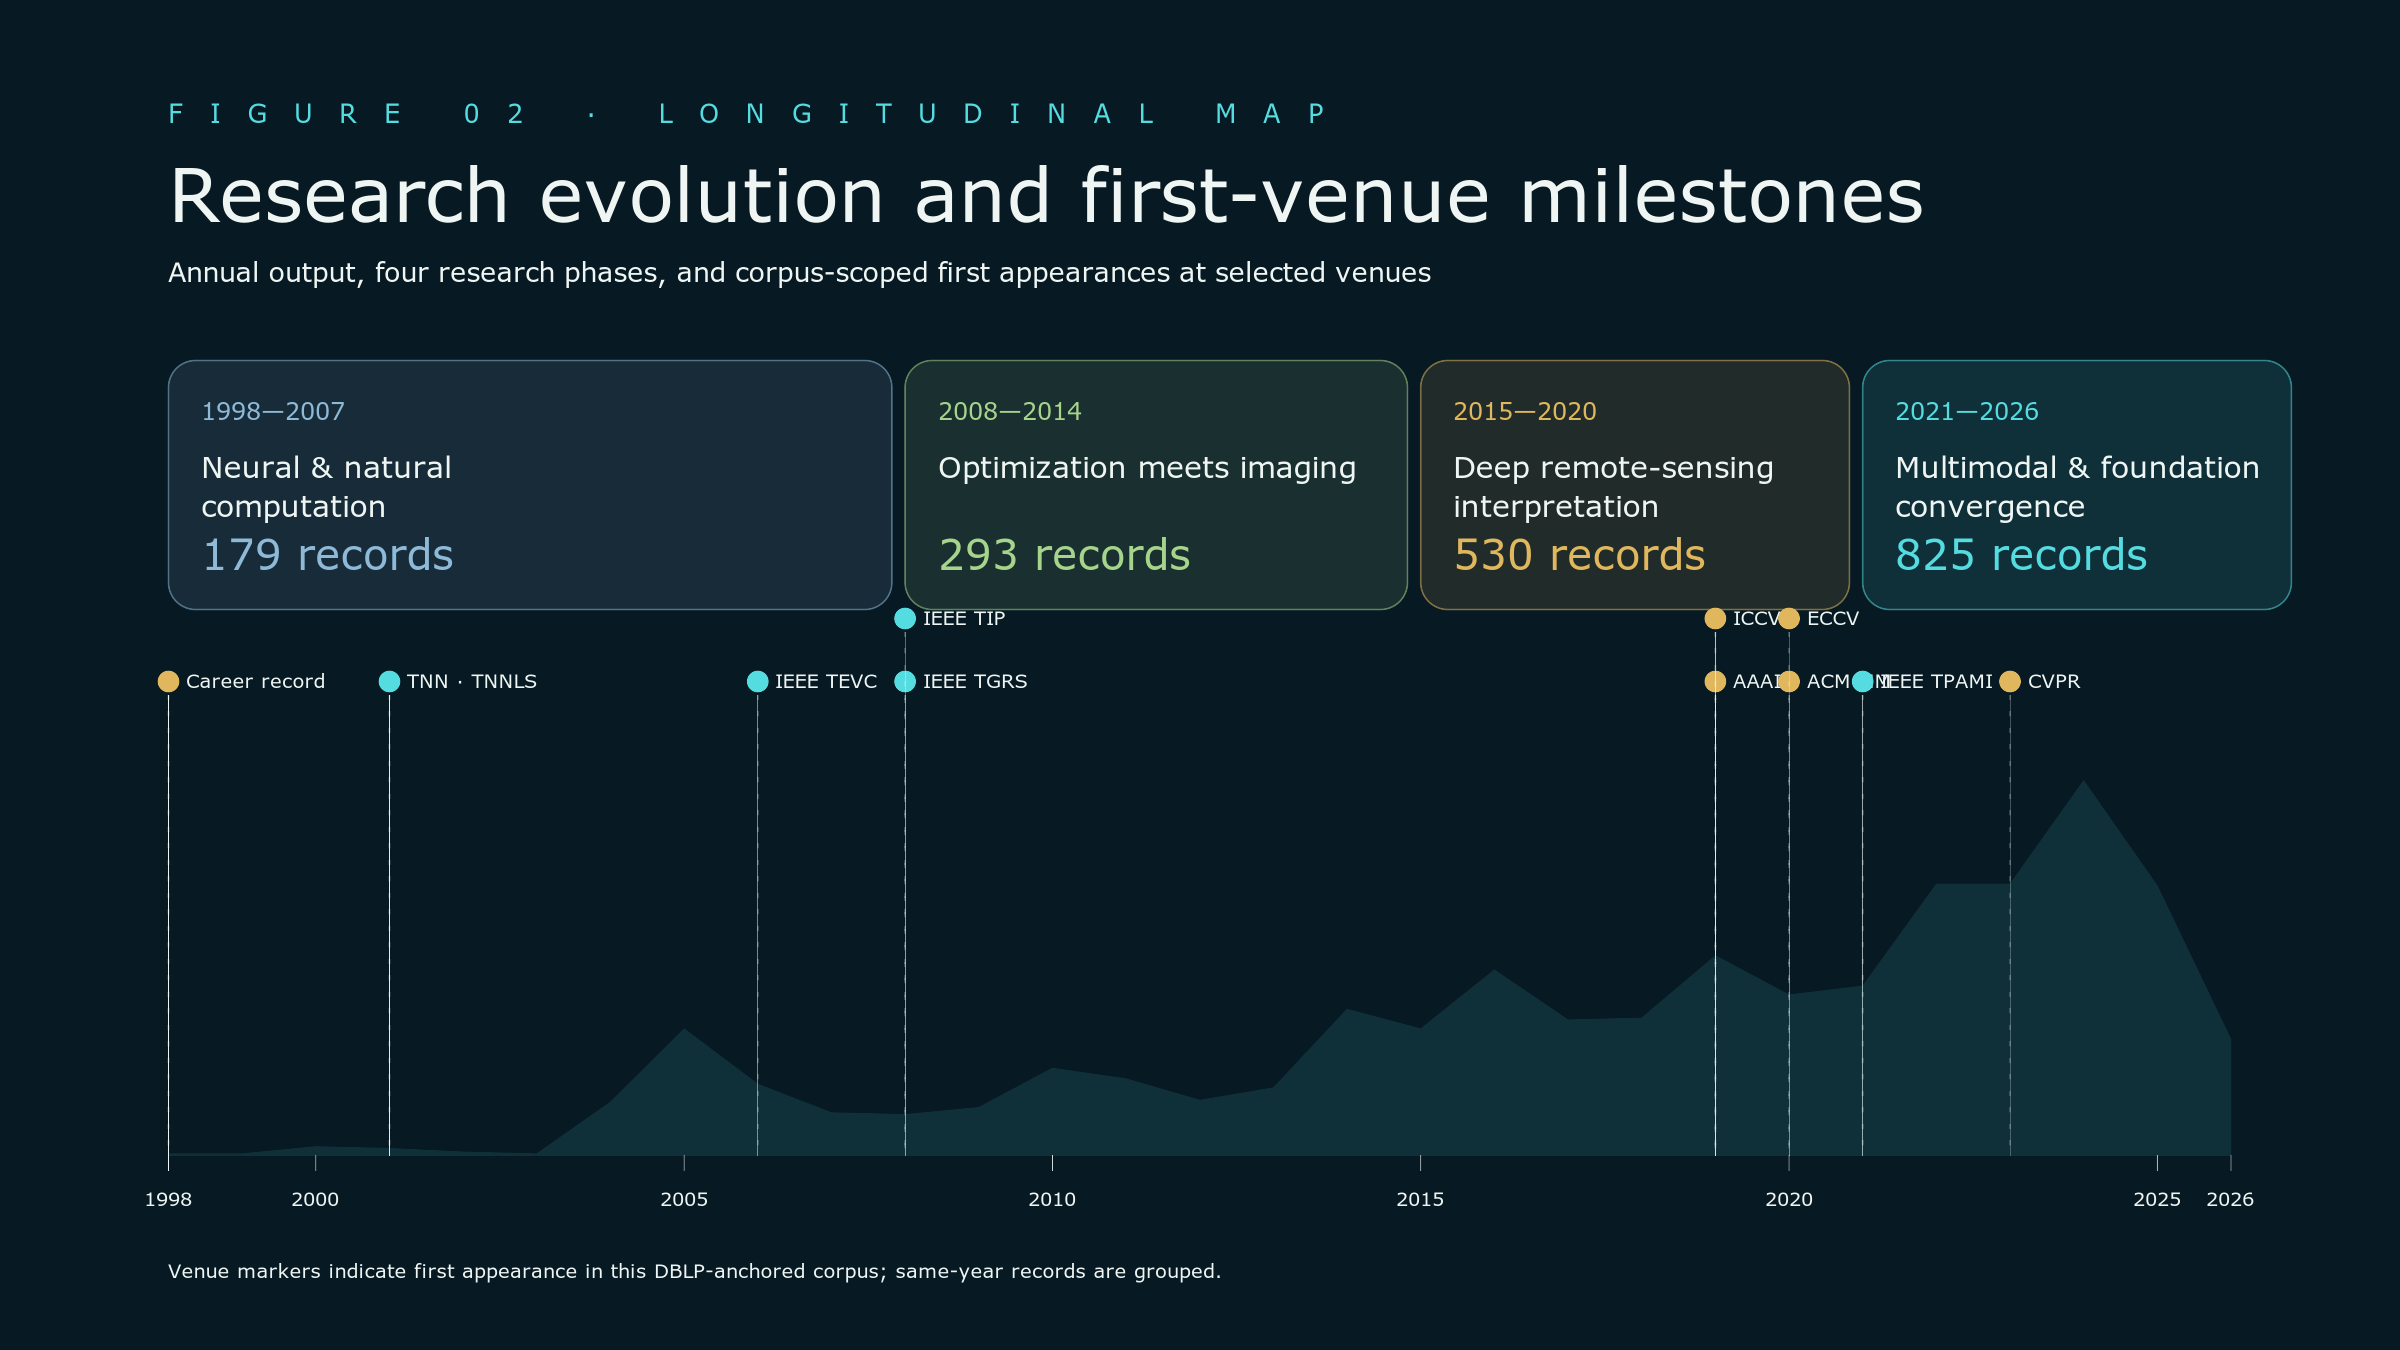
\includegraphics[width=\linewidth,alt={Timeline from 1998 to 2026 showing four phases, annual publication volume, and first appearances of selected venues in the public corpus.}]{figures/research-evolution-timeline.png}
\caption{Research evolution and selected first-venue milestones. Markers denote
the first appearance in the current DBLP-anchored corpus, not a claim about
records outside the dataset.}
\label{fig:evolution}
\figureqr{research-evolution timeline}{research-evolution-timeline}
\end{figure}

\subsection{Selected corpus-scoped first appearances}

Table~\ref{tab:firsts} records selected venue coordinates. The focus is not
prestige ranking. The ledger makes institutional expansion visible and gives
readers concrete entry points into the bibliography.

\begin{longtable}{>{\raggedright\arraybackslash}p{0.9cm}
                  >{\raggedright\arraybackslash}p{3.2cm}
                  >{\raggedright\arraybackslash}p{9.2cm}}
\caption{Selected first appearances in the current DBLP-anchored corpus.}
\label{tab:firsts}\\
\toprule
Year & Venue coordinate & First-year record or records \\
\midrule
\endfirsthead
\toprule
Year & Venue coordinate & First-year record or records \\
\midrule
\endhead
1998 & Corpus start & Total least mean squares algorithm \\
2001 & IEEE TNN / TNNLS & Multiwavelet neural network and its approximation properties \\
2002 & Pattern Recognition & Linear programming support vector machines \\
2005 & NeurIPS / NIPS & Response Analysis of Neuronal Population with Synaptic Depression \\
2006 & IEEE TEVC & An organizational coevolutionary algorithm for classification \\
2008 & IEEE TIP & Wavelet-Based Bayesian Image Estimation \\
2008 & IEEE TGRS & Spectral Clustering Ensemble Applied to SAR Image Segmentation \\
2019 & AAAI & Multi-Precision Quantized Neural Networks via Encoding Decomposition of \{-1,+1\} \cite{sun2019aaai} \\
2019 & ICCV & AFD-Net; and Better and Faster: Exponential Loss for Image Patch Matching \cite{quan2019iccv} \\
2019 & IJCAI & Accelerated Incremental Gradient Descent using Momentum Acceleration with Scaling Factor \\
2020 & ACM MM & A Novel Object Re-Track Framework for 3D Point Clouds \cite{feng2020acmmm} \\
2020 & ECCV & Supervised Edge Attention Network for Accurate Image Instance Segmentation \cite{chen2020eccv} \\
2021 & IEEE TPAMI & Accelerated Variance Reduction Stochastic ADMM for Large-Scale Machine Learning \cite{zheng2021tpami} \\
2023 & CVPR & Curvature-Balanced Feature Manifold Learning; and an online self-training study for semantic segmentation \cite{ma2023cvpr,zhao2023cvpr} \\
2023 & ICLR & Delving into Semantic Scale Imbalance \\
\bottomrule
\end{longtable}

\section{Hierarchical Thematic Architecture}

\begin{figure}[H]
\centering
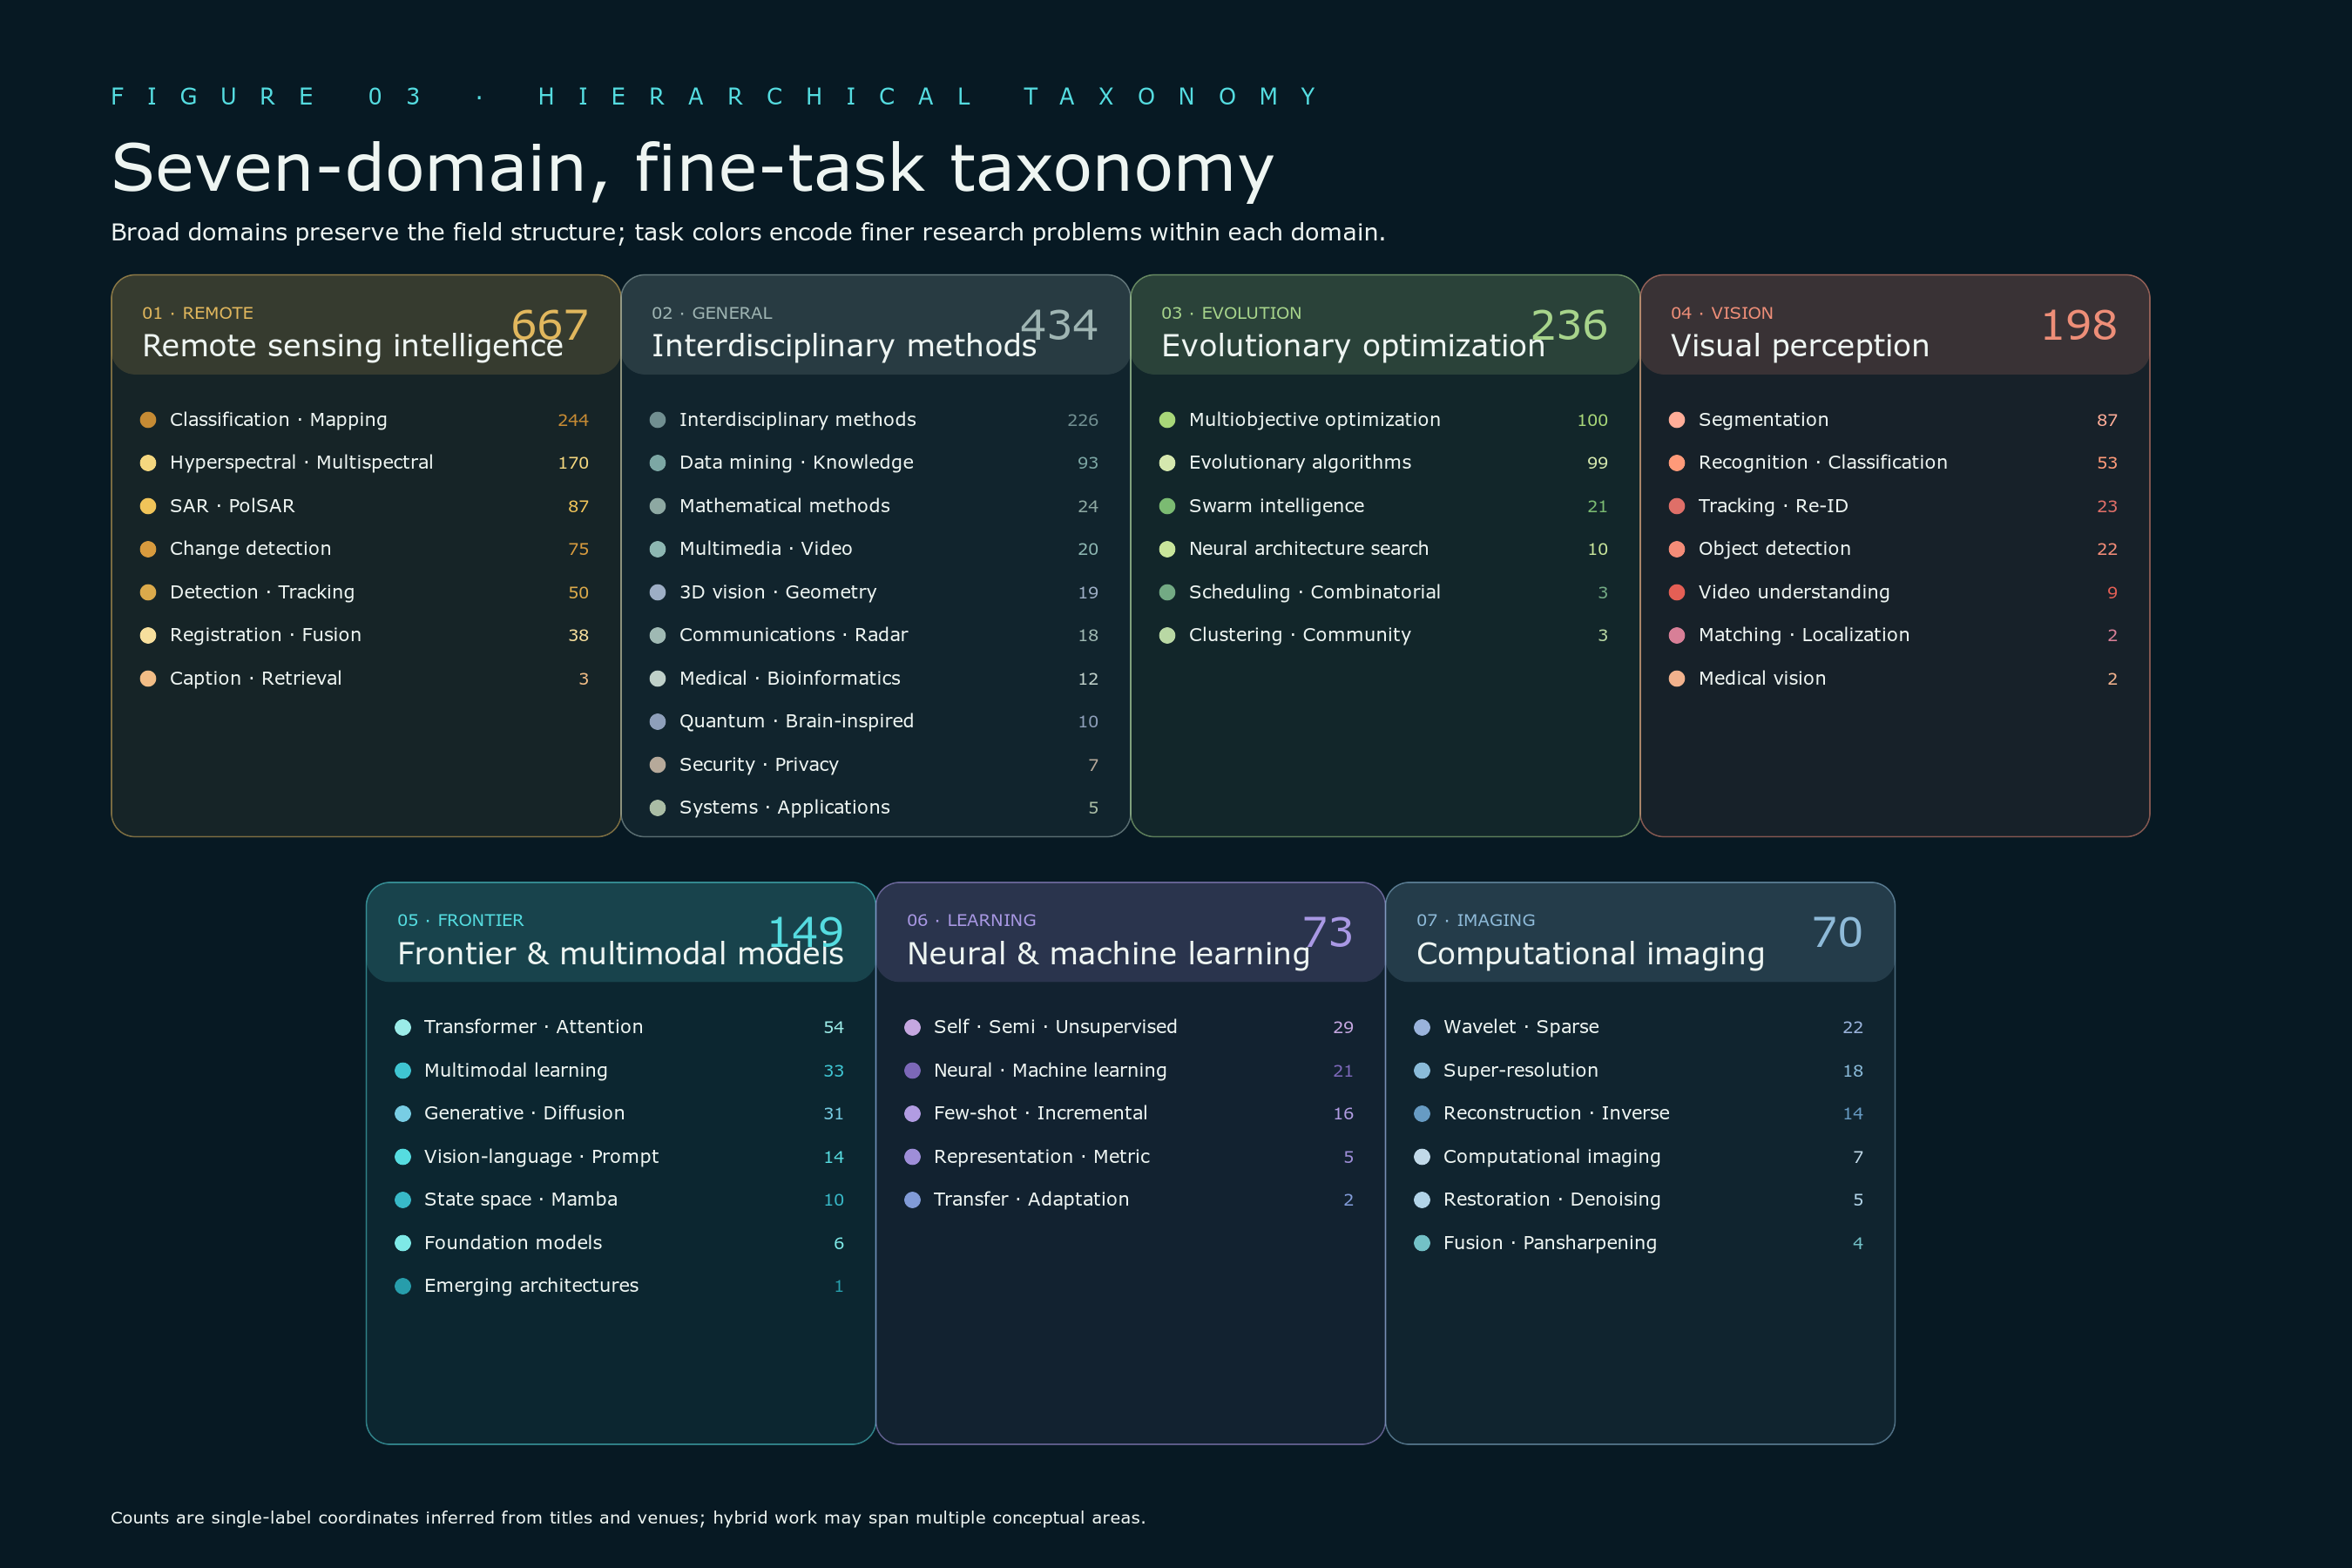
\includegraphics[width=\linewidth,alt={Seven-domain taxonomy showing fine-task labels and record counts for remote sensing, interdisciplinary methods, evolutionary optimization, visual perception, frontier models, neural learning, and computational imaging.}]{figures/hierarchical-task-taxonomy.png}
\caption{Hierarchical thematic map. Task colors are variations within each
domain family, matching the interactive paper graph. Counts are title-level,
single-label coordinates.}
\label{fig:taxonomy}
\figureqr{hierarchical task-taxonomy}{hierarchical-task-taxonomy}
\end{figure}

\subsection{Remote-sensing interpretation}

Remote sensing is the largest single-label domain with 667 records. Its internal
tasks include scene and land-cover classification, hyperspectral and
multispectral learning, SAR/PolSAR, change detection, object detection and
tracking, registration and fusion, and remote-sensing captioning. The count is
large enough to demonstrate a persistent domain core, but the cross-layer
framework cautions against treating it as an isolated application silo.

\subsection{Interdisciplinary methods}

The interdisciplinary domain contains 434 records in communications, medical
and bioinformatics applications, data mining, mathematical methods, security,
3D geometry, multimedia, and other systems. This category is intentionally
conservative: it receives records for which another broad domain is not the
strongest title-level coordinate. It therefore combines genuine
interdisciplinary reach with residual classification uncertainty.

\subsection{Evolutionary optimization}

Evolutionary and intelligent optimization contributes 236 records. The task
hierarchy separates multiobjective and many-objective optimization, general
evolutionary algorithms, swarm intelligence, neural architecture search,
clustering, transfer and multitask evolution, and combinatorial optimization.
The domain's influence is broader than the standalone count because search
methods reappear inside feature selection, architecture design, and remote
sensing.

\subsection{Visual perception}

Visual perception contains 198 records. Segmentation is the largest assigned
task, followed by recognition and classification, tracking and
re-identification, detection, video understanding, matching and localization,
and medical vision. Related visual work is also assigned to remote sensing and
frontier models, so this count is a lower bound on visual perception's role in
the full corpus.

\subsection{Frontier, learning, and imaging methods}

Frontier-model work contains 149 records, including Transformer and attention
architectures, multimodal learning, diffusion and generative models,
vision--language prompting, state-space models, and foundation models. Neural
and machine learning contributes another 73 records focused on self-,
semi-, and unsupervised learning; few-shot and incremental learning;
representation learning; and domain adaptation. Signal and computational
imaging contributes 70 records in wavelets, sparse representations,
reconstruction, super-resolution, restoration, denoising, and fusion.

\begin{table}[ht]
\centering
\caption{Broad thematic domains produced by the transparent title-level taxonomy.}
\label{tab:domains}
\begin{tabular}{lr}
\toprule
Domain & Records \\
\midrule
Remote-sensing interpretation & 667 \\
Interdisciplinary methods and applications & 434 \\
Evolutionary and intelligent optimization & 236 \\
Visual perception and understanding & 198 \\
Frontier models and multimodality & 149 \\
Neural and machine learning & 73 \\
Signal and computational imaging & 70 \\
\bottomrule
\end{tabular}
\end{table}

\section{Collaboration and Venue Ecology}

The corpus contains 2,163 normalized coauthor names. The highest collaboration
frequencies are Fang Liu (433 records), Shuyuan Yang (297), Lingling Li (249),
Xiangrong Zhang (245), Xu Liu (238), Biao Hou (237), Ronghua Shang (177),
Shuang Wang (158), Wenping Ma (138), and Yangyang Li (135). These repeated
relationships connect optimization, remote sensing, imaging, and visual
learning, but record counts cannot determine contribution or supervision.

\begin{figure}[H]
\centering
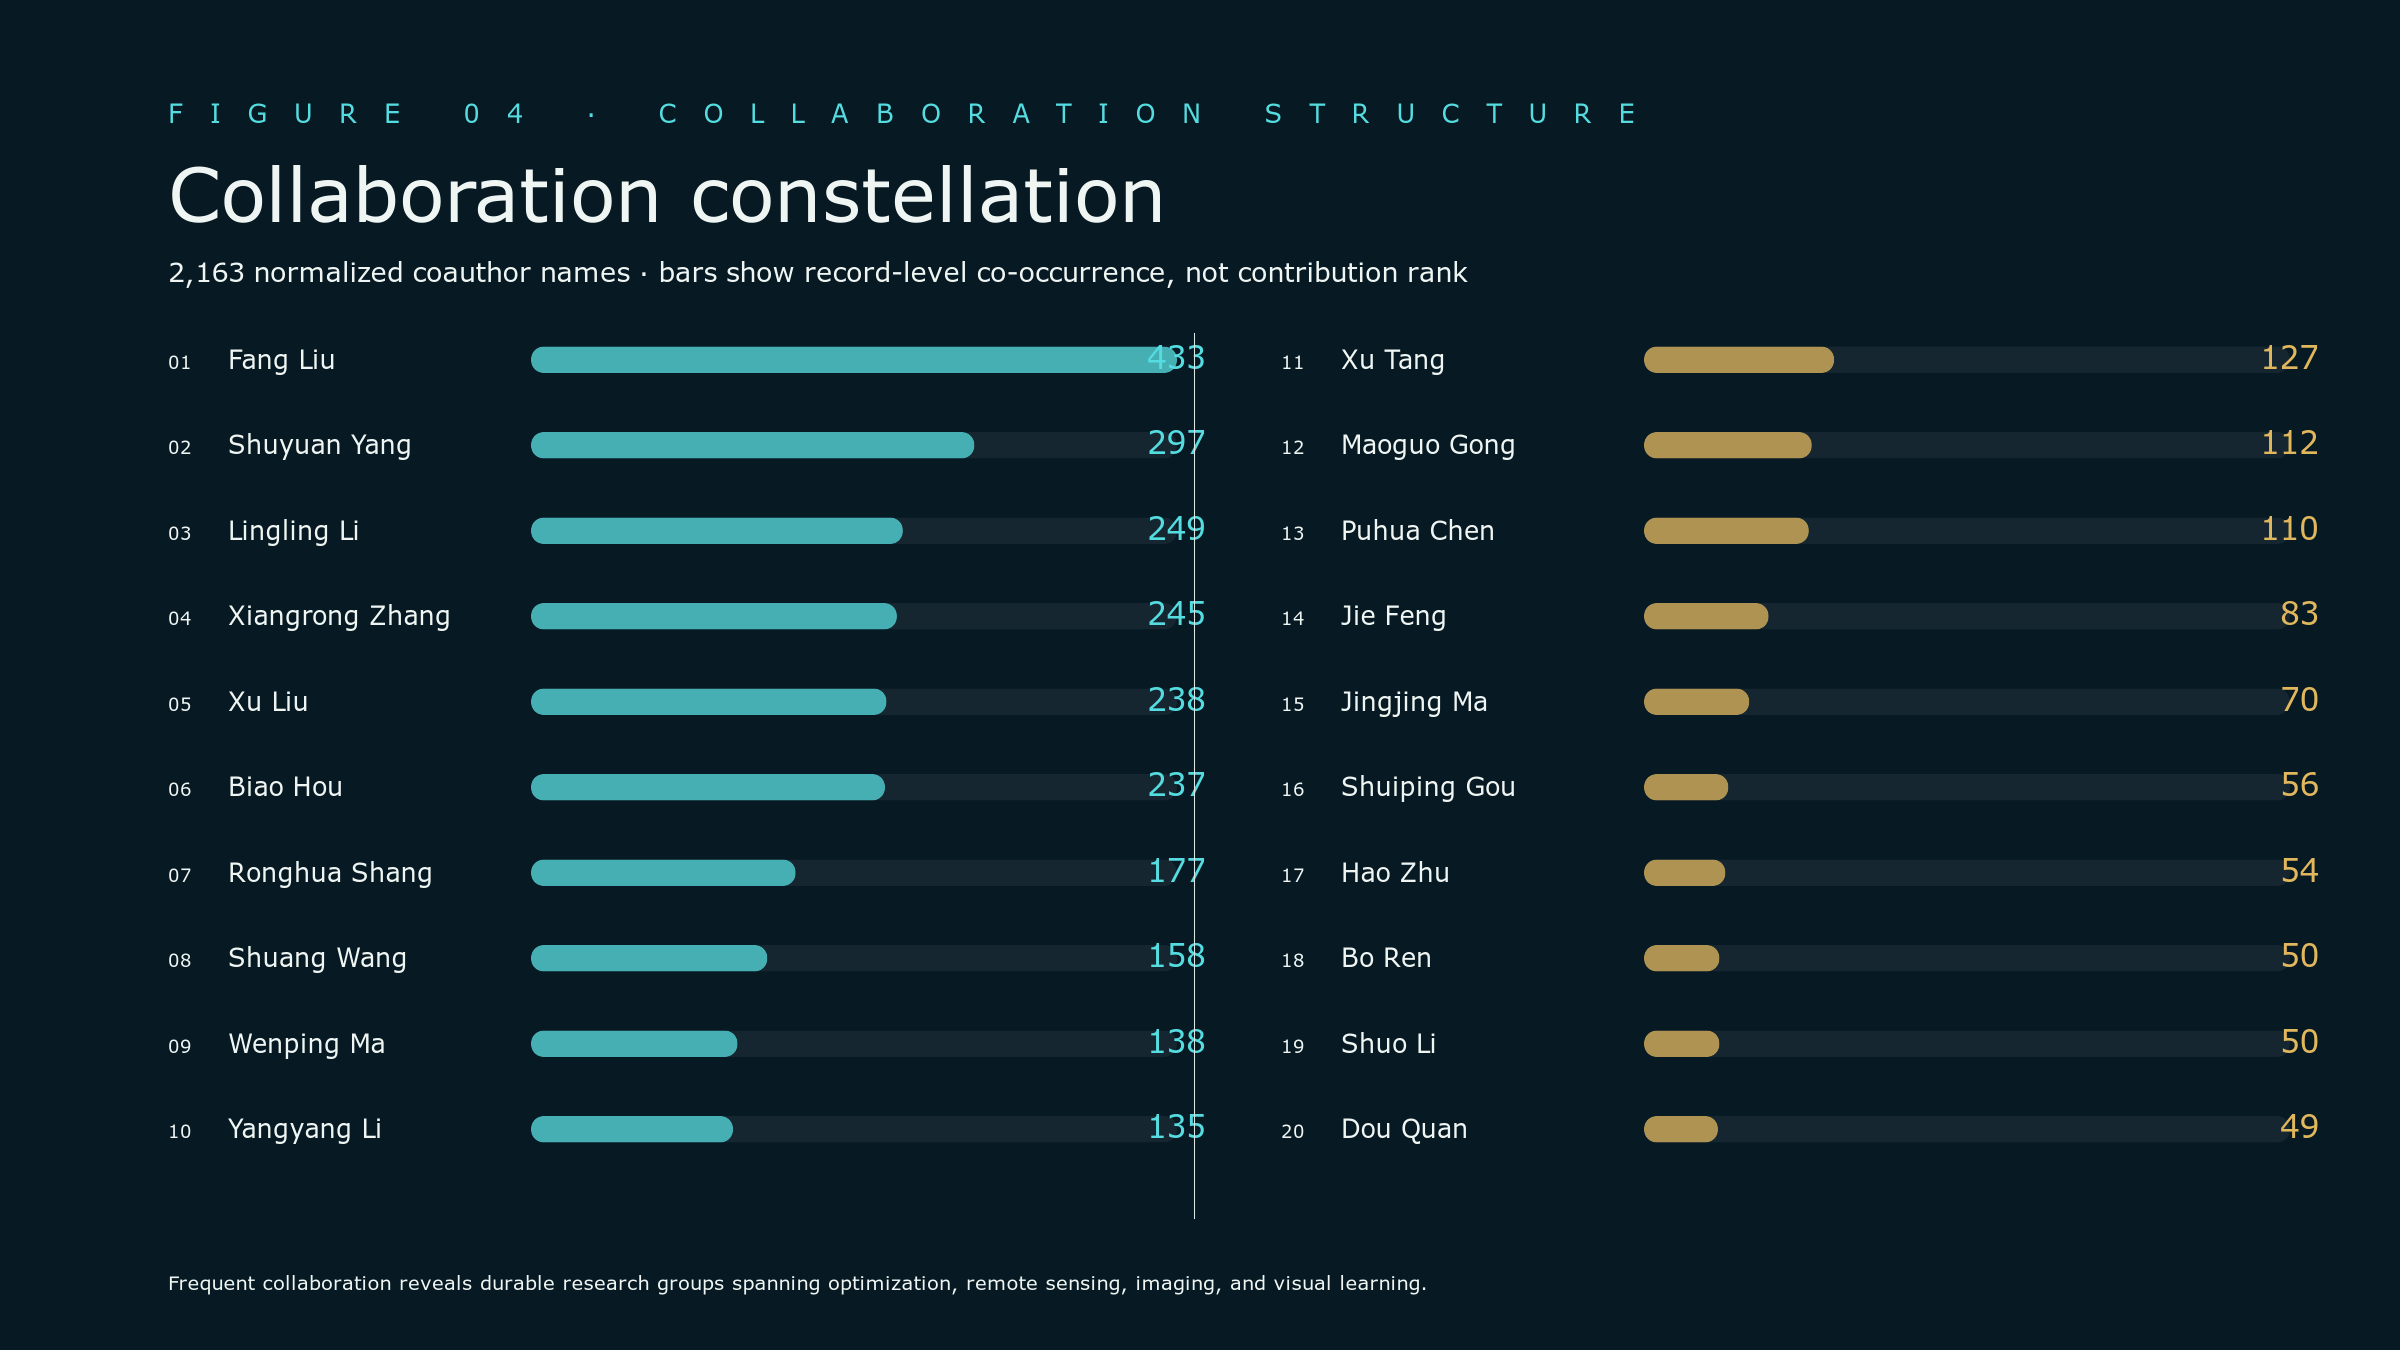
\includegraphics[width=\linewidth,alt={Horizontal bar chart ranking the twenty most frequent coauthors by number of corpus records shared with Licheng Jiao.}]{figures/collaboration-constellation.png}
\caption{Top twenty coauthor names by record-level co-occurrence. The complete,
searchable list is available in the interactive Atlas.}
\label{fig:collaboration}
\figureqr{collaboration-ranking}{collaboration-constellation}
\end{figure}

Venue concentration reinforces the thematic story. The most frequent sources
are \emph{IEEE Transactions on Geoscience and Remote Sensing} (255 records),
CoRR (125), IGARSS (104), \emph{IEEE Journal of Selected Topics in Applied
Earth Observations and Remote Sensing} (83), \emph{IEEE Geoscience and Remote
Sensing Letters} (71), \emph{Remote Sensing} (69),
\emph{Neurocomputing} (66), and \emph{Pattern Recognition} (63). The mixture
of archival journals, major conferences, and preprints reflects both a stable
domain core and rapid uptake of new methods.

\section{Impact Structure}

Of 1,764 DOI-bearing records, 1,682 matched the current Crossref Cited-by
snapshot. Raw citation rankings favor older publications and are sensitive to
database coverage. The Atlas preserves the raw count while adding a
publication-year cohort layer. A record is highlighted when it reaches the top
decile of its year cohort with at least five citations. A stronger landmark
layer requires the year-specific 99th percentile and at least 100 citations.

\begin{figure}[H]
\centering
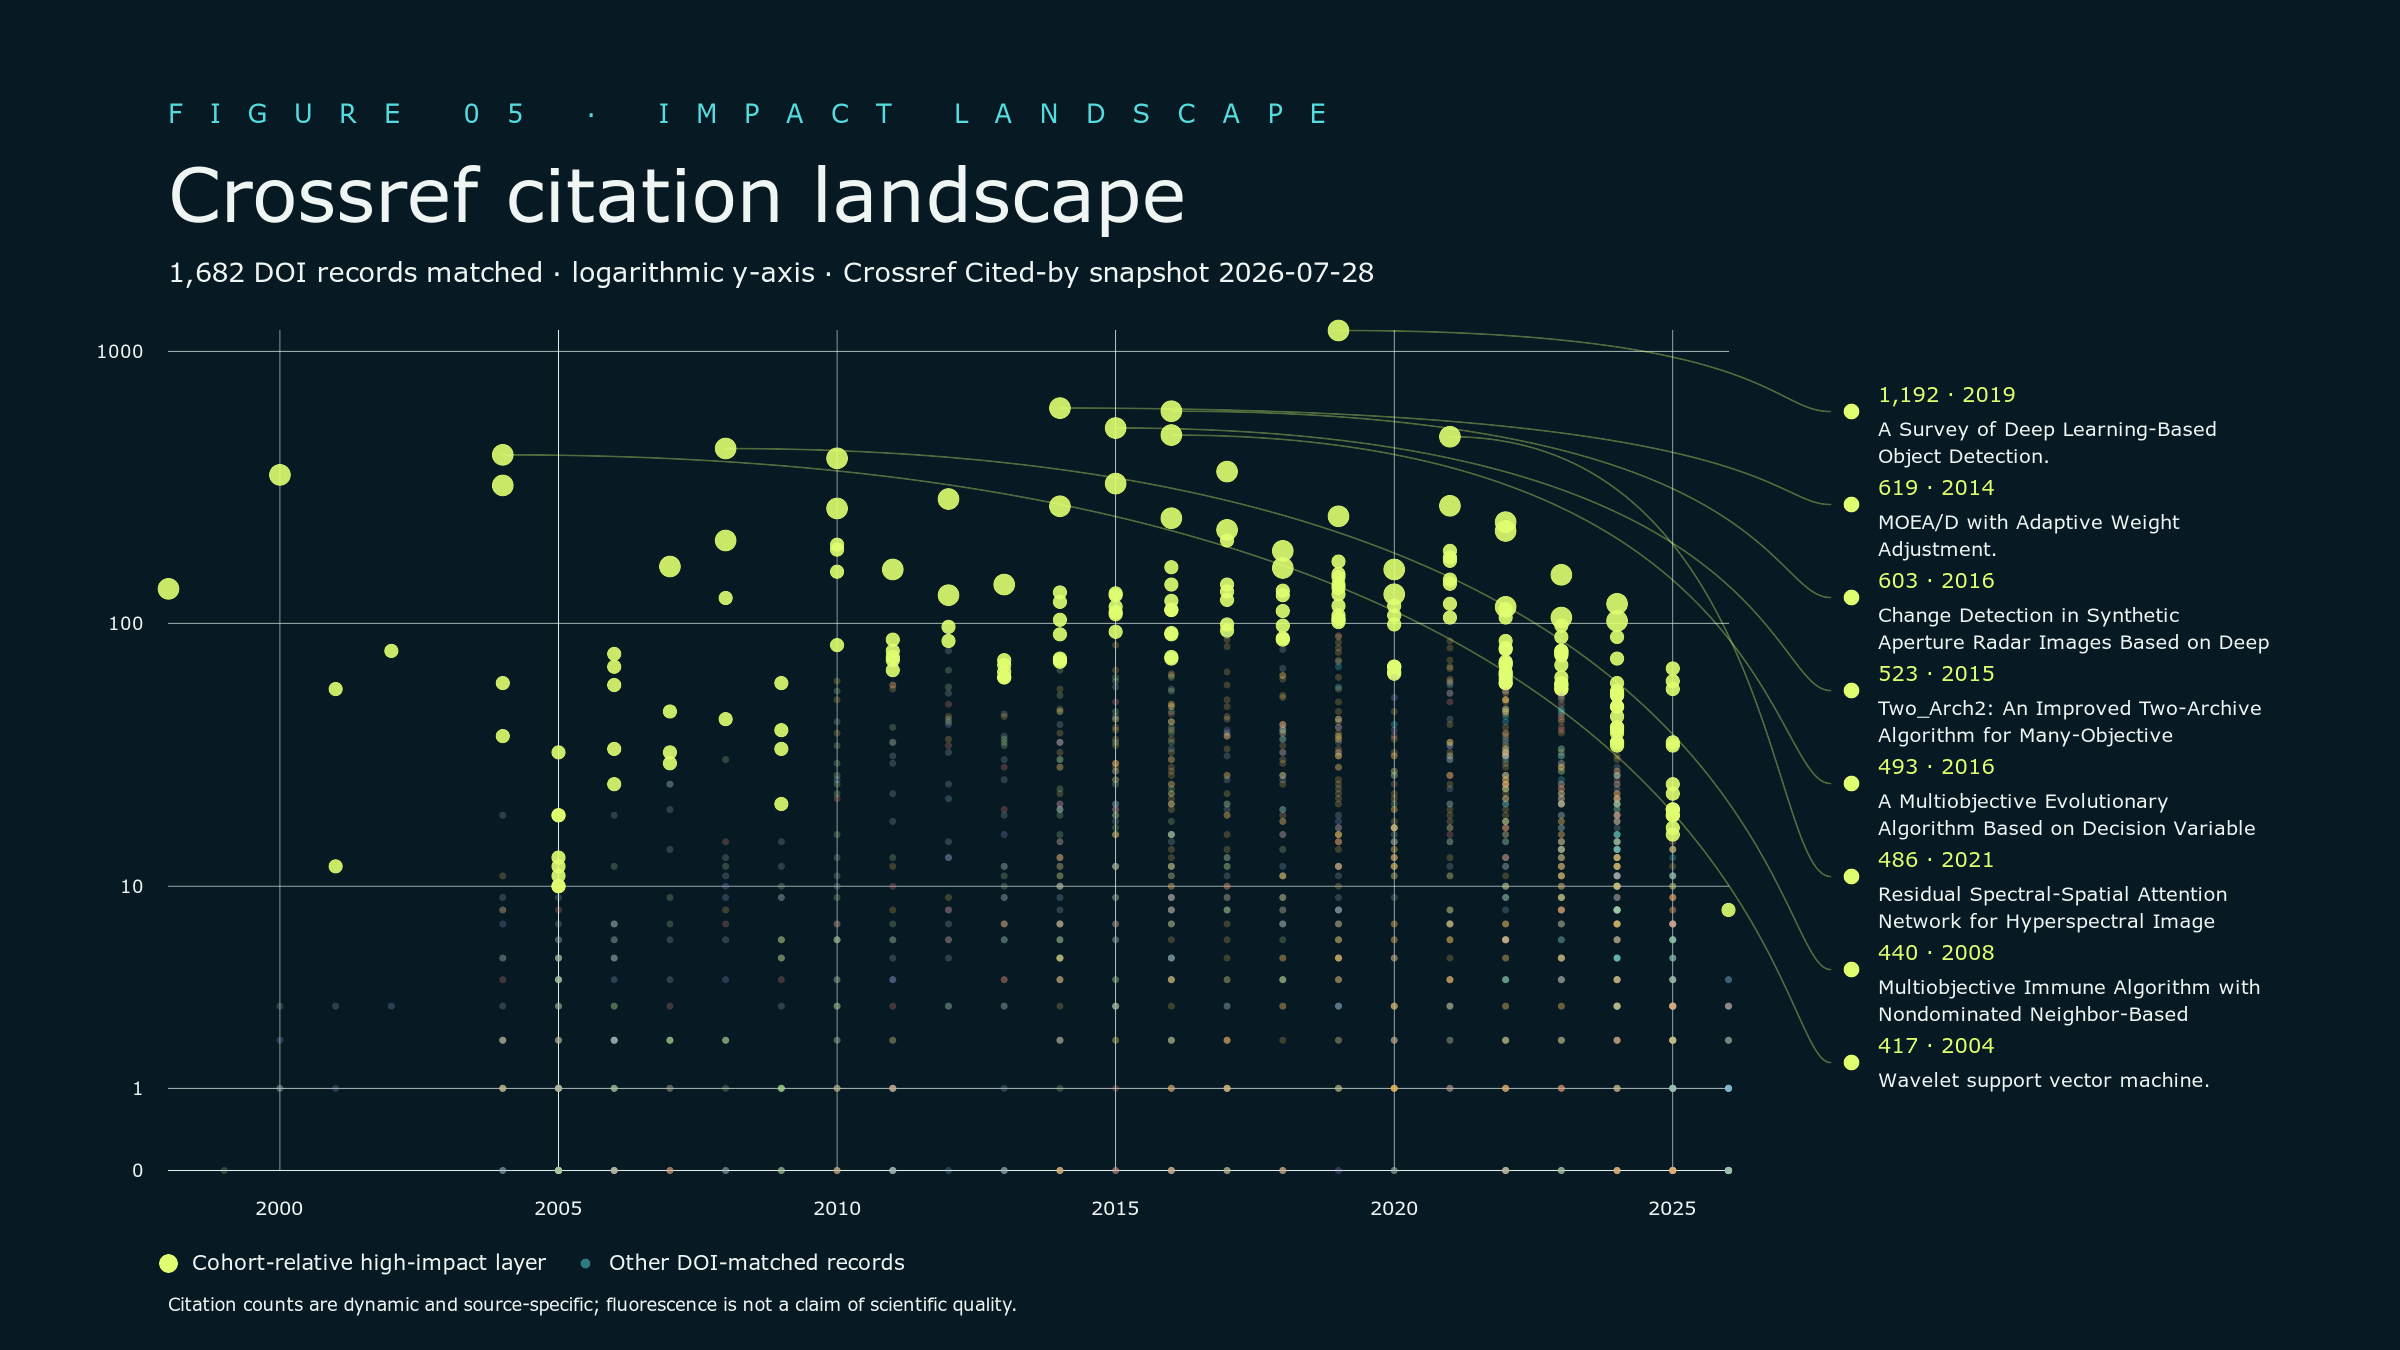
\includegraphics[width=\linewidth,alt={Scatter plot of publication year against logarithmic Crossref citation count, with cohort-relative high-impact papers highlighted and the eight highest counts annotated.}]{figures/citation-impact-landscape.png}
\caption{Crossref citation landscape. Fluorescence identifies unusually visible
records relative to their publication-year cohort; it is not a claim of
scientific quality.}
\label{fig:impact}
\figureqr{citation-impact landscape}{citation-impact-landscape}
\end{figure}

\begin{longtable}{r r p{0.62\linewidth}}
\caption{Highest Crossref Cited-by counts among DOI-matched corpus records,
updated 28 July 2026. Counts are dynamic and source-specific.}
\label{tab:high-cited}\\
\toprule
Citations & Year & Record \\
\midrule
\endfirsthead
\toprule
Citations & Year & Record \\
\midrule
\endhead
1,192 & 2019 & A Survey of Deep Learning-Based Object Detection
\cite{jiao2019objectdetection} \\
619 & 2014 & MOEA/D with Adaptive Weight Adjustment
\cite{qi2014moead} \\
603 & 2016 & Change Detection in Synthetic Aperture Radar Images Based on
Deep Neural Networks \cite{gong2016sarchange} \\
523 & 2015 & Two\_Arch2: An Improved Two-Archive Algorithm for
Many-Objective Optimization \cite{wang2015twoarch} \\
493 & 2016 & A Multiobjective Evolutionary Algorithm Based on Decision
Variable Analyses for Problems With Large-Scale Variables
\cite{ma2016largevariables} \\
486 & 2021 & Residual Spectral-Spatial Attention Network for Hyperspectral
Image Classification \cite{zhu2021ressan} \\
440 & 2008 & Multiobjective Immune Algorithm with Nondominated
Neighbor-Based Selection \cite{gong2008immune} \\
417 & 2004 & Wavelet Support Vector Machine \cite{zhang2004waveletsvm} \\
405 & 2010 & Adaptive NN Backstepping Output-Feedback Control for
Stochastic Nonlinear Strict-Feedback Systems With Time-Varying Delays
\cite{chen2010backstepping} \\
362 & 2017 & Remote Sensing Image Registration With Modified SIFT and
Enhanced Feature Matching \cite{ma2017registration} \\
352 & 2000 & A Novel Genetic Algorithm Based on Immunity
\cite{jiao2000immune} \\
327 & 2015 & A Novel Point-Matching Algorithm Based on Fast Sample
Consensus for Image Registration \cite{wu2015pointmatching} \\
\bottomrule
\end{longtable}

Citation counts should never be treated as a direct measure of scientific
quality. Their strongest role here is navigational: they identify records that
warrant close reading and help compare visibility across topics and years.

\section{Cross-Cutting Synthesis}

Three recurring mechanisms reconnect the thematic map.

\begin{enumerate}
\item \textbf{Structure-aware representation.} Multiscale transforms, sparse
representations, spectral--spatial relations, geometric constraints, attention,
and state-space models all encode structure rather than treating feature
learning as undifferentiated.
\item \textbf{Search, selection, and adaptation.} Evolutionary search,
multiobjective optimization, feature selection, transfer, prompting, and
architecture search repeatedly address how a model or solution process should
adapt to a task.
\item \textbf{Method--domain coevolution.} Remote sensing is not merely an
application destination. Its multiscale, multimodal, geometric, and physically
grounded problems repeatedly motivate new representations and optimization
formulations.
\end{enumerate}

These mechanisms explain why the contemporary frontier is better described as
accumulation and recombination than as disconnected trend following.
Transformer, vision--language, diffusion, prompt, Mamba, and foundation-model
papers appear inside a program already organized around structured signals,
adaptive search, and demanding perception domains.

\section{Open Questions}

The current map motivates five questions for a deeper full-text review.

\begin{enumerate}
\item \textbf{How does domain structure enter modern foundation models?}
Source-level analysis should distinguish architectural encoding, data
construction, objectives, prompting, and post-training adaptation.
\item \textbf{Where does evolutionary search create unique value?} Comparative
reading is needed to separate shared mechanisms from inherited terminology
across classical evolutionary computation, architecture search, and prompt or
model adaptation.
\item \textbf{How do representations move across sensors and tasks?}
Version-linked experiments could reveal when representations developed for
SAR, hyperspectral, change detection, or matching transfer to other modalities.
\item \textbf{Can impact be measured beyond raw citations?} Future releases
should combine source-verified references, citation contexts, benchmark
adoption, code availability, and field-normalized indicators.
\item \textbf{How does collaboration mediate research evolution?}
Affiliation-aware and author-disambiguated analysis could test how methods,
domains, and venue frontiers travel across teams and generations.
\end{enumerate}

\section{Limitations and Reproducibility}

The evidence base supports corpus mapping, descriptive bibliometrics,
title-level thematic coding, collaboration counts, corpus-scoped venue firsts,
and source-labeled citation analysis. It does not support claims about
experimental results, causal influence, intellectual priority, or a paper's
technical contribution beyond verified metadata.

Conference, preprint, and journal versions may coexist. Author-name
normalization cannot resolve every homonym. Crossref coverage is incomplete and
dynamic. A deterministic one-label taxonomy can misclassify hybrid work.
``First'' means first appearance in the selected DBLP-anchored dataset, not an
absolute career claim.

Reproducibility assets include the public field allowlist, taxonomy rules,
milestone generator, citation-refresh script, figure generator, QR assets,
semantic HTML, this LaTeX manuscript, and the compiled PDF. The analysis can
therefore be extended incrementally as verified abstracts, full text,
references, and affiliations become available. The HTML and LaTeX follow
arXiv's guidance on semantic structure and alternative descriptions
\cite{arxiv-accessible-html,arxiv-latex-html}.

\section{Conclusion}

The 1998--2026 record portrays a research program with unusual continuity
across neural computation, evolutionary optimization, image intelligence, and
remote sensing. Its contemporary work on multimodal and foundation models is
not an isolated turn; it extends longstanding interests in structured
representation, adaptive search, and complex visual signals. The open Atlas
and this systematic map provide a transparent baseline for source-verified
technical synthesis, reference-network analysis, and reusable scholarly tools.

\bibliographystyle{plain}
\bibliography{references}

\end{document}
